\documentclass[openany,oneside]{book}

\usepackage{jluthesisUTF8}
%\usepackage{gbt7714}
\usepackage{amsmath}
\usepackage{fontspec}

%%%%%%从这一行以下所有的包都不是模版所必须的,可以根据需要选用
\usepackage{amssymb, amsfonts}
\usepackage{mathrsfs}
\usepackage{amsthm}
\usepackage{enumerate}
\usepackage{graphicx}
\usepackage{tikz}
\usepackage{multirow}
\usepackage{lipsum}
\usepackage{graphicx}
\usepackage{tabularx}
\usepackage{listings}
\usepackage{pgf}
%\usepackage{cite}

%\usetikzlibrary{arrows}
\usepackage{xeCJK}

\newtheoremstyle{cthmstyle}%〈name〉
{3pt}%〈Space above〉
{3pt}%〈Space below〉
{\kai}%〈Body font〉
{}%〈Indent amount〉
{\bf}%〈Theorem head font〉
{.}%〈Punctuation after theorem head〉
{.5em}%〈Space after theorem head〉
{}%〈Theorem head spec(can be left empty, meaning ‘normal’)〉
\theoremstyle{cthmstyle}
\newtheorem{thm}{定理}
\newtheorem{lem}{引理}
\newtheorem{cor}{推论}
\newtheorem{prop}{命题}

\newtheorem*{thm*}{定理}
\newtheorem*{lem*}{引理}
\newtheorem*{cor*}{推论}
\newtheorem*{prop*}{命题}

\theoremstyle{definition}
\newtheorem{defn}{定义}
\newtheorem*{defn*}{定义}

\theoremstyle{remark}
\newtheorem{rem}{注释}
\newtheorem*{rem*}{注释}
\newtheorem{example}{例}
\newtheorem*{example*}{例}

\renewcommand{\proofname}{\rm\kai 证明}

%opening
\hypersetup{
    pdftitle  = {your pdf title},
    pdfsubject  = {your pdf subject},
    pdfkeywords = {your pdf keywords},
    pdfauthor   = {your name}
}


\begin{document}

\frontmatter
\sloppy % 解决中英文混排的断行问题,会加入间距,但不会影响断行 ????

%
% 手动在长标题中利用 \par 输入断行,
\ctitle{一个因为某些机缘巧合变得冗长\par 而又枯燥的中文标题~~~~~~~~}
\etitle{O Serendipity, You Made This English Title~~~~~~\par Tediously Long~~~~~~~~}
                                       % 论文 内容提要
\cthesissummary{
    中文摘要。
}
%                                           % 关键词
\ckeywords{甲, 乙, 丙}

\ethesissummary {
    Engligh abstract goes here.
}

\ekeywords{a, b, c}

\cdate{2021年5月17日}
\cauthor{张~~三}

\makecover


\pagenumbering{Roman} 
%\pdfbookmark[0]{目~~~~录}{contents}

\tableofcontents
{\xiaosi}
%{\fontsize \fontsize{12.05pt}{14.45pt}\selectfont}
% 清除目录后面空页的页眉和页脚
\clearpage{\pagestyle{empty}\cleardoublepage}

%%% 正文
\mainmatter
\defaultfont                        % 正文使用默认字体,小四,宋体

\chapter{绪论}

可用cite去引用。\cite{dean2008mapreduce, marxapplication}

\lipsum



\chapter{一级标题}

一级标题

\section{二级标题}

{\hei 二级标题}

\subsection{三级标题}

三级标题

\subsubsection{四级标题}

四级标题

\chapter{例子}

\section{公式,定理及证明}

下面是\cite{bzj2006constcurative}中性质2的推论。

\begin{cor}
设$C:\mathbb R\to \mathbb R^3$是具有常曲率$k\ne 0$的曲线。那么对于任何满足\[p^5+16p\cdot q+ \sum_{i=1}^{\infty} \mathrm{Li}(pq)\cdot\left(\frac {\zeta(q-p)} {i!}\right)^i = 0\]的$p$和$q$,方程$f(x)=x^3+px+q$都有五个根。
\end{cor}

\begin{proof}
假设结论不成立,那么由曲线基本定理存在一条曲线$\gamma$使得$\gamma(t)$处的的曲率为$1$,但挠率为$\sin t$。但这与\cite{bzj2006constcurative}中的性质2矛盾。
\end{proof}

\begin{rem*}
同样的方法也可以用于证明$(V=L)$蕴含强不可达基数$\kappa$的存在性。
\end{rem*}


\section{图像}
\subsection{tikz}

\def\R{\mathbb R}
\begin{center}
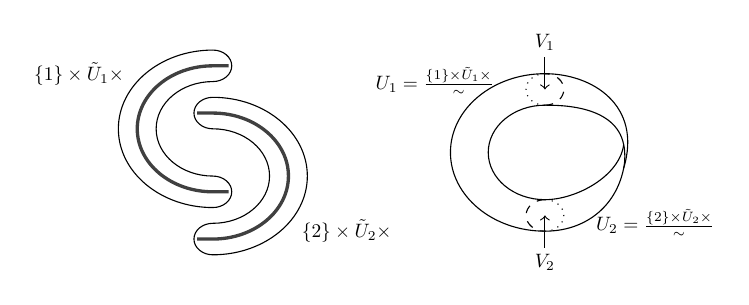
\begin{tikzpicture}
    \begin{scope}
        %\viewaxisgrid[0.5]{1.9};
        
        \draw (0,1.3) arc (90:270:1.2 and 1.0);
        \draw[very thick,darkgray] (0.2,1.1) -- (0,1.1) arc (90:270:0.96 and 0.8) -- (0.2,-0.5);
        \draw (0,0.9) arc (-90:90:0.24 and 0.2);
        \draw (0,0.9) arc (90:270:0.72 and 0.6);
        \draw (0,-0.7) arc (-90:90:0.24 and 0.2);
        
        \draw (0,-1.3) arc (-90:90:1.2 and 1.0);
        \draw[very thick,darkgray] (-0.2,-1.1) -- (0,-1.1) arc (-90:90:0.96 and 0.8) -- (-0.2,0.5);
        \draw (0,-0.9) arc (90:270:0.24 and 0.2);
        \draw (0,-0.9) arc (-90:90:0.72 and 0.6);
        \draw (0,0.7) arc (90:270:0.24 and 0.2);
        
        \node [scale=0.7] at (-1.7,1.0) {$\{1\} \times \tilde U_1\times \R$};
        \node [scale=0.7] at (1.7,-1.0) {$\{2\} \times \tilde U_2\times \R$};
    \end{scope}
    
    \begin{scope}[xshift=120]
        %\viewaxisgrid[0.5]{1.9};
        
        \draw (0,1.0) arc (90:270:1.2 and 1.0);
        \draw[dashed] (0,0.6) arc (-90:90:0.24 and 0.2);
        \draw (0,0.6) arc (90:270:0.72 and 0.6);
        \draw[dotted] (0,-1.0) arc (-90:90:0.24 and 0.2);
        
        \draw (0,-1.0) .. controls +(0.5, 0.0) and +(-0.1,-0.5) .. 
               (1.0,-0.2) .. controls +(0.02,0.1) and +(0.02,-0.1) .. 
               (1.0,0.1) .. controls +(-0.1,0.5) and +(0.2,0.0) .. (0,0.6);
        \draw (0,-0.6) .. controls +(0.4,0.0) and +(-0.05,-0.4) .. (1.0,0.1);
        \draw (0,1.0)  .. controls +(0.6,0.0) and +(0.24,0.8) .. (1.0,-0.2);
        \draw[dashed] (0,-0.6) arc (90:270:0.24 and 0.2);
        \draw[dotted] (0,1.0) arc (90:270:0.24 and 0.2);
        
        \node [scale=0.7] at (-1.4,0.9) {$U_1 = \frac{\{1\}\times \tilde U_1\times \R}{\sim}$};
        \node [scale=0.7] at (1.4,-0.9) {$U_2 = \frac{\{2\}\times \tilde U_2\times \R}{\sim}$};
        \draw[->] (0.0,1.4)  node [fill=white, scale=0.7] {$V_1$} -- (0.0,0.8);
        \draw[->] (0.0,-1.4) node [fill=white, scale=0.7] {$V_2$} -- (0.0,-0.8);
    \end{scope}
\end{tikzpicture}
\end{center}

\subsection{pgf}

\begin{center}

\begin{tikzpicture}[blend group=screen]
  \fill[red!90!black]   ( 90:.6) circle (1);
  \fill[green!80!black] (210:.6) circle (1);
  \fill[blue!90!black] (330:.6) circle (1);
\end{tikzpicture}
\end{center}

\newpage
\section{列表}

没有序号的列表。
\begin{itemize}
\item 生产力决定生产关系
\item 经济基础决定上层建筑
\end{itemize}

有序号的列表。
\begin{enumerate}
\item 矛盾的同一性和斗争性
\item 矛盾的普遍性和特殊性
\item ...
\end{enumerate}

\section{表格}

\begin{center}
        \begin{tabular}{|c|c|c|c|}
        \hline
        \multicolumn{3}{|c|}{白天} & 晚上 \\ \hline
        吃饭     & 喝酒     & 打麻将    & 睡觉 \\ \hline
        很好     & 不好     & 一般     & 很好 \\ \hline
        \end{tabular}
\end{center}

%
\clearpage
%\rule{0ex}{0ex}
\section{富有启发性的思想}

\begin{quote}
    \begin{verse}
        我拿起烟斗装满叶烟,\\
        \hspace{1em}吞云吐雾消磨时光。\\
        人在那坐着,却飘走了思想------\\
        \hspace{1em}它飘向一幅画,晦黯而忧伤:\\
        \hspace{2em}那画告诉我这是多么相像,\\
        \hspace{2em}我和这烟斗一模一样。\\
        \vspace{1em}
        
        这喷香溢郁的烟斗同我相仿,\\
        \hspace{1em}都不过是尘芥不过是土壤;\\
        我最终也要归为尘灰。\\
        \hspace{1em}烟斗落地,没等听到声响,\\
        \hspace{2em}就已经拦腰摔断,不幸遭殃;\\
        \hspace{2em}相同的命运我也将承当。\par
        \vspace{1em}
        
        洁白的烟斗没有污斑,\\
        \hspace{1em}从未玷染,从未弄脏。\\
        可总有一天会命归无常, \\
        \hspace{1em}在草地下奄埋这副皮囊;\\
        \hspace{2em}我的肉体将变黑,一副晦暗相,\\
        \hspace{2em}就象这烟斗,若是它使用得经常。\\
        \vspace{1em}
        
        当烟斗被点燃,闪耀着火光,\\
        \hspace{1em}瞧,它们立刻就冒出青烟袅袅飘荡;\\
        轻烟散进空气,无处寻访,\\
        \hspace{1em}烟斗里便只剩有灰烬留藏。\\
        \hspace{2em}虚名也将消泯,正同那青烟一样,\\
        \hspace{2em}而躯体最终只不过化作上壤。\\
        \vspace{1em}
        
        吸烟时这种事也发生得经常:\\
        \hspace{1em}架上的塞烟器不翼而飞,给你添忙,\\
        这下你只好上手,虽然不很便当,\\
        \hspace{1em}可手指伸进烟锅,难免要被烫伤。\\
        \hspace{2em}既然烟斗里都有痛苦伏藏,\\
        \hspace{2em}地狱里的痛苦将会何其难当!\\
        \vspace{1em}
        
        由对烟斗的沉思,导向了别的玄想,\\
        \hspace{1em}沉溺在格致冥思中,\\
        也有益于身心的健康;\\
        \hspace{1em}这样吞云吐雾,心中着实舒畅,\\
        \hspace{2em}因此无论在国内、国外、陆地或海洋,\\
        \hspace{2em}我都要一边抽我的烟斗,一边坚定对上帝的信仰。\\
    \end{verse}
\end{quote}



%最后设置格式,插入参考文献。
\defaultfont
\bibliographystyle{./gbt7714-author-year} %用GBT7714-2015格式进行排版。若未安装此拓展包导致报错,可以将\bibliographystyle改为plain,如下一行所示
%\bibliographystyle{plain}
\clearpage
\phantomsection
\addcontentsline{toc}{chapter}{参考文献}
\nocite{*} %展示所有的参考文献,即使正文中没有显式引用过。如果不需要,请注释掉这一行。
\bibliography{document}
%插入致谢
\chapter*{致 \qquad 谢}
\addcontentsline{toc}{chapter}{致谢}
\thispagestyle{empty}

坚持实事求是,反对脱离历史条件的空谈蛮干。实事求是,也是历史唯物主义观点。历史主义和唯物主义是有机联系、浑然一体的。坚持历史主义,必须坚持唯物主义,必须反对官僚主义、主观臆断,反对虚无主义、神秘主义,反对一切形式的空想和蛮干。尊重客观形势、尊重客观实际,才能制定出符合规律的方针路线,我们的事业才能胜利,我们才能尽可能地少走弯路。“吃大锅饭”,就是过高地估计了人民群众的思想素质和道德素质,在没有严格的规章制度、科学的预算和纪律要求的保障下,采取了过于理想的社会模式,从而使得很多道德水平低下的人消积怠工、投机取巧,使得许多管理水平低下的人走上领导者岗位,加上某些别有用心的人煽动、破坏,给我们的事业造成了巨大损失。

认清历史形势,利用一切有利条件和时机,敢于变革,推动人类社会向更高的物质文明和精神文明发展。坚持历史唯物主义观念,也要防止那些“教条主义、保守主义”等呆板运用历史唯物主义观点的行为。不能清醒地认清形势和历史发展趋势,不敢变革或不愿变革,也可能坐失发展良机,给以后的事业造成难以挽回的损失。比如在当今竞争日趋激烈、形势日趋复杂、能源日益紧张、不稳定因素大量存在、腐败势力十分强大、道德认识存在多元化矛盾化等等情况下,如果不能高瞻远瞩、未雨绸缪,及早采取加强国防、反腐倡廉、利民惠民、统一思想、加强德育、发展周边的关系等一系列果断措施,必然会给我们的事业带来难以控制的损失。

\end{document}
